\subsection{任务描述}

如图\ref{fig:construction_of_tec8},各个部件控制信号可以通过微程序控制器生成或通过硬布线控制器生成。实验要求小组成员通过使用HDL自行设计硬布线控制器的逻辑,以实现一个可以正常工作的CPU。
硬布线控制器需要根据输入产生正确的控制信号,其中各输入分别为IR7 ~ IR4、W3~W1、CLR、SWCBA、C、Z、T,输入信号意义详见表\ref{tab:output_signal},硬布线控制器输出为各个控制信号。各个输入信号
和输出信号已经与硬布线控制器对应引脚连接,其对应关系如图\ref{fig:pins}所示

\begin{figure}[htbp]
    \centering
    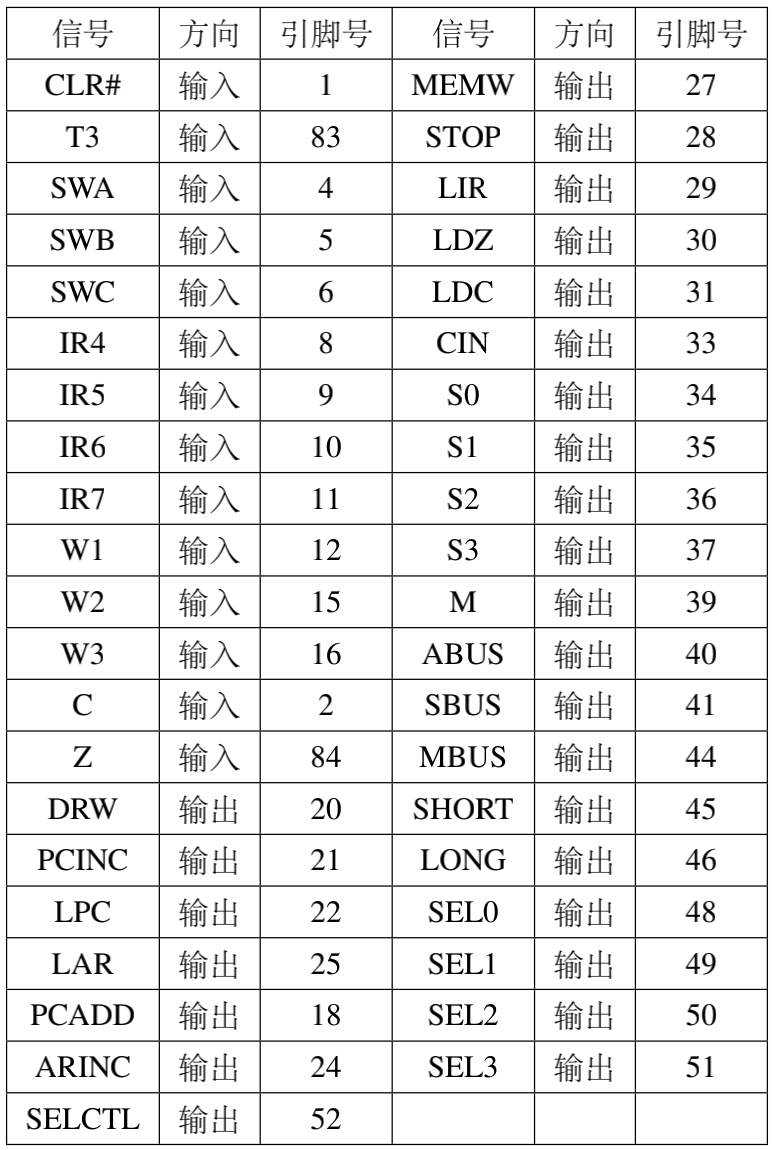
\includegraphics{figures/chapter1/pins.png}
    \caption{引脚规定}
    \label{fig:pins}
\end{figure}

\newpage
\subsubsection{题目一}

基于Altera EPM7128进行设计,完成一个顺序模型处理机。
\begin{itemize}
    \item 基本功能
    \begin{enumerate}
        \item 实现读写寄存器
        \item 实现读写存储器
        \item 实现基本指令操作
    \end{enumerate}
    \item 附加功能
    \begin{enumerate}
        \item 拓展三条及以上指令
        \item 实现在执行程序前设置PC
    \end{enumerate}
\end{itemize}

基本指令表如图\ref{fig:instruction}所示。

\begin{figure}[htbp]
    \centering
    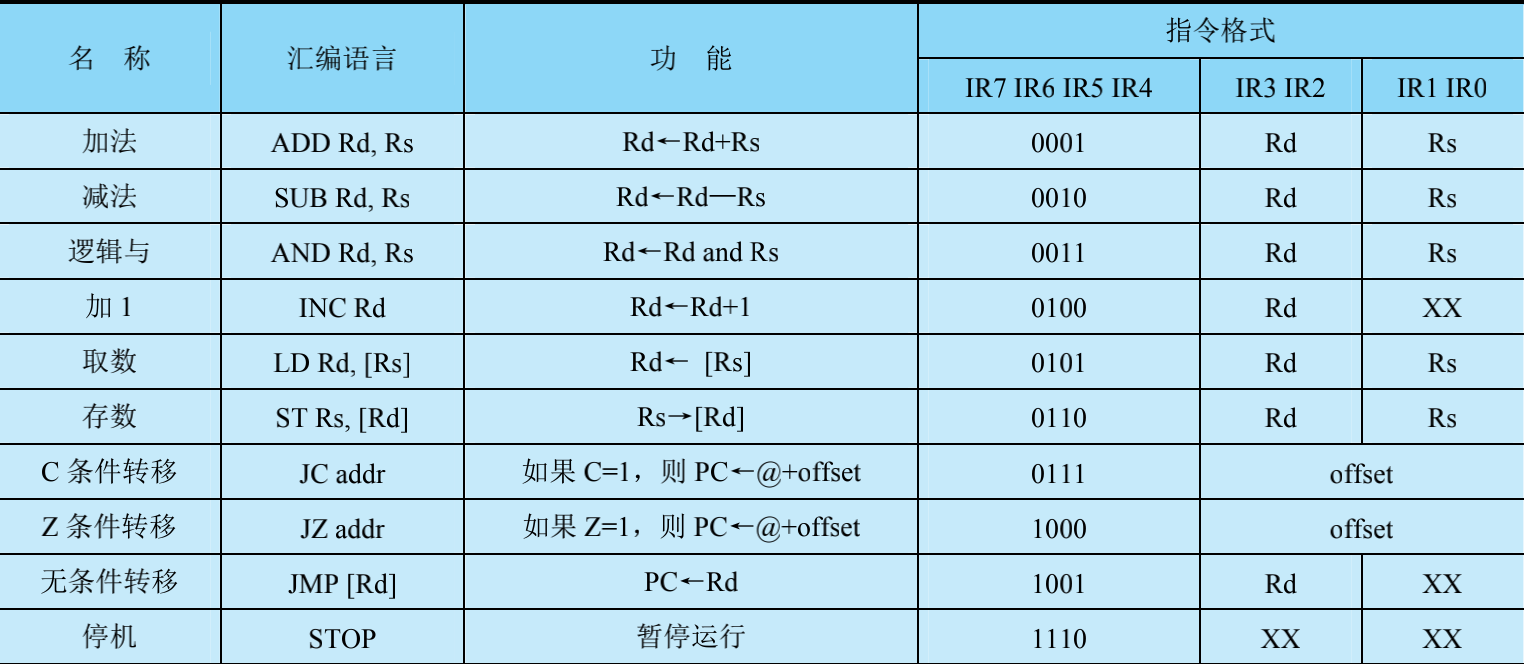
\includegraphics[width=0.9\linewidth]{figures/chapter1/instruction.png}
    \caption{基本指令}
    \label{fig:instruction}
\end{figure}

\subsubsection{题目二}
在题目一的基础上,将顺序执行的硬布线控制器改为流水线控制器以提高运行效率,并在TEC-8上完成组装、调试运行。

\subsubsection{题目三}
基于TEC-8系统完成中断功能硬布线控制器设计。


